\documentclass{article}
\usepackage{geometry}
\usepackage{array}
% \usepackage[a4paper, margin=1.2in]{geometry}
\usepackage{hyperref}
\usepackage{makeidx}
\usepackage{biblatex}
\usepackage{dsfont}
\usepackage{amsmath}
\usepackage{amssymb}
\usepackage{fancyhdr}
\usepackage{algorithm}
\usepackage{algpseudocode}
\usepackage{graphicx} % Required for inserting images

\graphicspath{./images/}
\bibliography{references}

\DeclareMathOperator*{\argmax}{arg\,max}

\makeindex

\pagestyle{fancy}
\fancyhf{}

\lhead{Reinforcement Learning}
\rhead{Balaji Karedla}
\fancyfoot[C]{\thepage}

\title{\textbf{Reinforcement Learning} \\ SoS MidTerm Report}
\author{Balaji Karedla}
\date{June 2024}

\hypersetup{
    colorlinks=true,       % Set to true to use colored links instead of boxes
    linkcolor=black,        % Color for internal links (sections, table of contents)
    filecolor=magenta,     % Color for file links
    urlcolor=cyan,         % Color for external links
    citecolor=blue,        % Color for citation links
    linkbordercolor={0 0 0}, % Set link border color to black (effectively hides the box)
    pdfborder={0 0 0}      % Remove link borders (set to 0 0 0 to remove all borders)
}

\begin{document}

\maketitle

\pagenumbering{roman}

\tableofcontents

\newpage

\pagenumbering{arabic}

\section{Introduction}
% \begin{center}
%     \textbf{\Huge{Edit it Later!!!}}
% \end{center}

% As I embarked on my journey into the realm of machine learning, one area that particularly captured my interest was reinforcement learning (RL). This subset of machine learning stands out because of its unique approach to training algorithms through interaction with an environment. Unlike supervised learning, which relies on a vast dataset of labeled examples, reinforcement learning focuses on learning optimal behaviors through trial and error.

% In reinforcement learning, an agent learns to make decisions by performing actions in a given environment to achieve a specific goal. To draw a simple analogy, consider playing a video game. Here, the agent represents the player, and the environment corresponds to the game world. The player's objective is to make moves that score points or advance levels. Through continuous interaction with the game, the player gradually learns which actions yield the highest scores or successfully complete the levels.

% This learning process is driven by the concept of rewards and punishments. The agent receives feedback from the environment in the form of rewards (positive feedback) or penalties (negative feedback) based on its actions. Over time, the agent aims to maximize its cumulative reward by identifying and executing actions that yield the most favorable outcomes. This method of learning closely mimics the way humans and animals learn from their surroundings, making it a compelling area of study.

% Reinforcement learning has already demonstrated its potential in various domains, from game playing (such as AlphaGo and OpenAI's Dota 2 bot) to robotics, autonomous driving, and even financial trading. Its ability to adapt and improve through interaction makes it a powerful tool for tackling complex decision-making problems.

% As I continue to explore this fascinating field, I am eager to delve deeper into the algorithms and techniques that drive reinforcement learning. Understanding these foundational concepts is the first step towards leveraging RL to develop intelligent systems capable of making informed and autonomous decisions.

This is the report of my project on Reinforcement Learning as a part of Summer of Science 2024 by the Mathematics and Physics (MnP) Club.

This is a branch of Machine Learning along with Supervised and Unsupervised Learning. In Supervised Learning, the model is trained on a labeled dataset, while in Unsupervised Learning, the model just goes through the dataset without any labels.

Reinforcement Learning differs from the both as it learns from the environment by interacting with it. The agent learns to achieve a goal by trying out stuff, getting rewards or punishments, and learning from time to time.

Reinforcement Learning is therefore close to how humans learn from their surroundings. But the way human learns from the environment is too complex and not yet understood completely. But, the RL algorithms are designed to mimic the way humans learn.

This is what made me feel interested in Reinforcement Learning. The work I did in this project is present in the \href{https://github.com/balaji1029/reinforcement-learning-sos/}{repo} on GitHub. The graphs I plotted, the code I wrote are all present in the repo. The code is written in Python and the libraries used are \texttt{numpy} and \texttt{matplotlib}.
\section{Multi-Armed Bandits (MAB)}

% Multi-Armed Bandits are common in casinos and are one of the easily modelled games in Reinforcement Learning. The name "Multi-Armed Bandit" comes from the slot machines in casinos, also known as one-armed bandits. The slot machines have a lever (arm) the player pulls to play the game. The player can choose from multiple slot machines with a different reward distribution. The goal is to maximize the total reward by selecting the slot machine with the highest expected reward. The player faces a trade-off between exploring different slot machines to learn their reward distributions and exploiting the best-known slot machine to maximize the reward. This trade-off is known as the exploration-exploitation dilemma.

Multi-Armed Bandits are common in casinos and are one of the most basic problems in Reinforcement Learning. The slot machines have levers (arms), which the player pulls to play the game.The player is rewarded according to the arm pulled. The  The goal, just like any other game, is to maximize the total reward by selecting the arms accordingly.

\begin{figure}[h]
    \centering
    \includegraphics[width=0.5\linewidth]{images/mab.png}
    \caption{A Slot Machine or an Armed Bandit}
    \label{fig:mab}
\end{figure}

The Multi-Armed Bandit I studied is a simple version of the Reinforcement Learning problem, where an agent interacts with an environment by selecting one of the available actions (arms) at each time step.

I chose a 10-armed bandit from \cite{sutton2018reinforcement}, where the mean of the rewards given by the bandit was randomly selected over a constant distribution over a $[-2,2)$ range. The bandits give a reward chosen from a normal distribution with a mean equal to the mean of the bandit and a standard deviation of $1$. The agent aims to maximize the total reward by selecting the bandit with the highest expected reward.

\subsection{Agent Implementation}

I implemented the agent using the different algorithms given in~\cite{sutton2018reinforcement}. The implementation in all of these algorithms included storing an array of action values, which are estimates of the expected rewards of each bandit. The agent selects the action with the highest action value to \textit{exploit}, the best-known bandit, or selects a random action to \textit{explore} other bandits. The agent updates the action values based on the rewards received from the environment.

The updation of the action values is different across different algorithms.

\subsection{Greedy Algorithm}

The Greedy Algorithm is the simplest Algorithm for solving the Multi-Armed Bandit problem. The agent keeps track of the action values for each bandit and selects the bandit with the highest action value at each time step. The agent \textit{exploits} the best-known bandit by choosing the action with the highest action value.

The action values of the bandits, represented by $q_{\ast}$, are estimated by the agent using the sample average method to get an estimate, represented by $Q_t$. The action value of a bandit $a$ at time step $t$ is updated using the following formula:
\[q_\ast\doteq \mathds{E} [R_t|A_t=a]\]
\[Q_t(a)\doteq \frac{\sum_{i=1}^{t-1} R_i \cdot \mathds{1}_{A_i=a}}{\sum_{i=1}^{t-1} \mathds{1}_{A_i=a}}\]

where $R_t$ is the reward received by the agent at time step $t$, $A_t$ is the action selected by the agent at time step $t$, and $\mathds{1}_{A_i=a}$ is an indicator function that is $1$ if $A_i=a$ and $0$ otherwise.

In the greedy algorithm, the agent always selects the bandit with the highest action value. So,

\[A_t \doteq \argmax_{a} Q_t(a)\]

This definition of $Q_t$ lets us define it recursively as follows:
\[Q_{t+1} = Q_t + \frac{1}{n}[R_t - Q_t]\]

where $n$ is the number of times the action $a$ has been selected.

\subsection{Exploration-Exploitation Dilemma}

The Greedy Algorithm has a drawback in that it always selects the bandit with the highest action value, which can lead to suboptimal performance. The agent may not explore other bandits to learn their reward distributions, which can result in a lower total reward.

This can be overcome by choosing a random bandit every time with equal probability to explore the bandits. This ensures the agent explores all the bandits and learns their reward distributions. But the reward is highly distributed, so the agent may be unable to exploit the best bandit.

This is the Exploration-Exploitation Dilemma in the Multi-Armed Bandit problem. This can be overcome by choosing the perfect ratio of exploration and exploitation.

\subsection{$\epsilon$-Greedy Algorithm}

The $\epsilon$-Greedy Algorithm is a simple solution to the Exploration-Exploitation Dilemma. The agent selects the best-known bandit with probability $1-\epsilon$ and selects a random bandit with probability $\epsilon$. The agent \textit{exploits} the best-known bandit with probability $1-\epsilon$ and \textit{explores} other bandits with probability $\epsilon$\footnote{Assuming there are $k$ bandits, the probability of selecting a bandit $a$ at time step $t$ is given by:
\[\pi(a_t=a|S_t) = \begin{cases}
    1-\epsilon + \frac{\epsilon}{k} & \text{if } a = \argmax_{a} Q_t(a) \\ \frac{\epsilon}{k} & \text{otherwise}
\end{cases}\]}.

The action value of a bandit $a$ at time step $t$ is updated using the following formula:
\[Q_{t+1}(a) = Q_t(a) + \frac{1}{n}[R_t - Q_t(a)]\]

where $n$ is the number of times the action $a$ has been selected.

The value of $\epsilon$ is a hyperparameter that controls the exploration and exploitation trade-off. A higher value of $\epsilon$ encourages more exploration, while a lower value of $\epsilon$ encourages more exploitation.

\begin{figure}[h!]
    \centering
    \includegraphics[width=0.75\linewidth]{images/compare-epsilon-greedy.png}
    \caption{The $\epsilon$-Greedy Algorithm}
    \label{fig:epsilon_greedy}
\end{figure}

The \ref{fig:epsilon_greedy} shows the performance of the $\epsilon$-Greedy Algorithm with different values of $\epsilon$. The performance of the algorithm is measured by the average reward over time. The algorithm with $\epsilon=0.1$ performs better than the algorithm with $\epsilon=0.01$ and $\epsilon=0$.

It is obvious that the greedy algorithm grows faster than the other algorithm at the beginning but the $\epsilon$-greedy algorithm with $\epsilon=0.1$ performs better than the greedy algorithm in the long run. The $\epsilon=0.01$ algorithm is closer to the greedy algorithm, but it performs better than the greedy algorithm in the long run, it even performs better than the $\epsilon=0.1$ algorithm in the long run, but it grows slower than the $\epsilon=0.1$ algorithm.

Completely random selection of bandits ($\epsilon=0$) performs the worst among all the algorithms. The agent does not exploit the best-known bandit and spends most of the time exploring other bandits, resulting in a lower total reward.

\begin{figure}[h!]
    \centering
    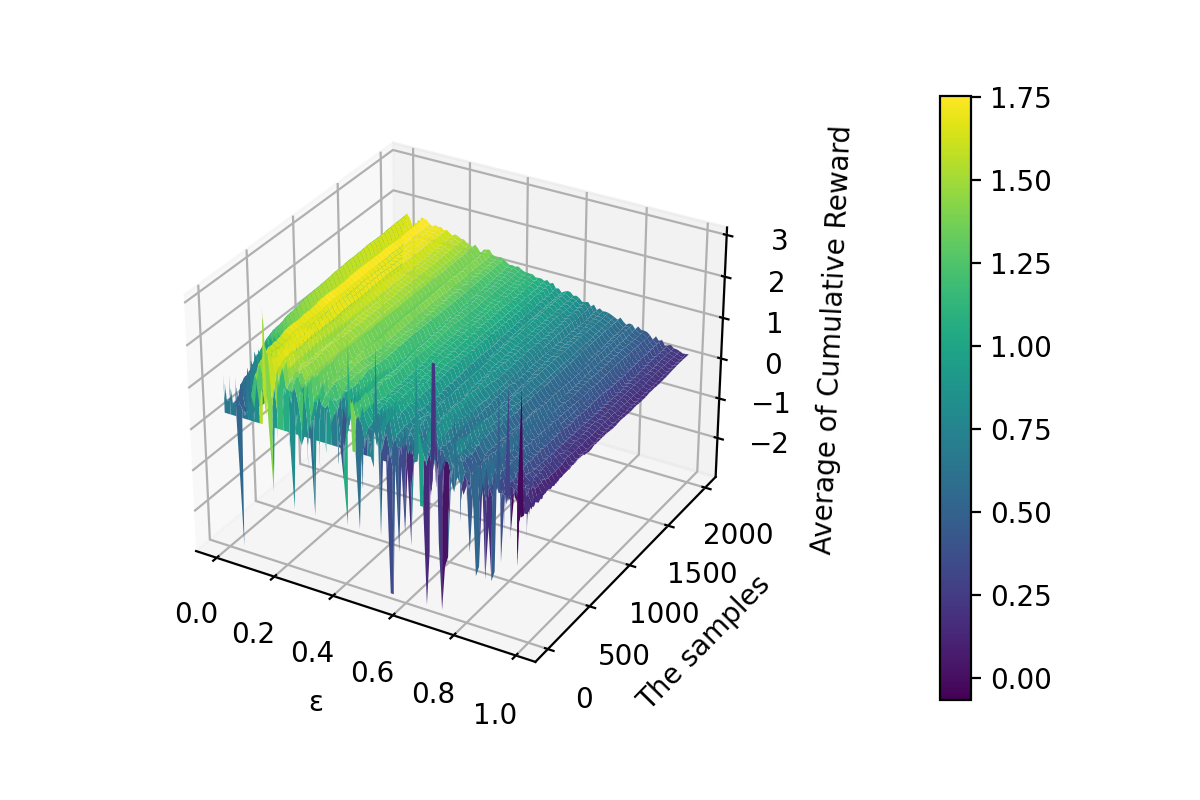
\includegraphics[width=0.49\linewidth]{images/3d-compare-epsilon-greedy.png}
    \includegraphics[width=0.49\linewidth]{images/compare-epsilons-greedy.png}
    \caption{Comparison of epsilons in the $\epsilon$-Greedy Algorithm}
    \label{fig:epsilon_greedy_optimistic}
\end{figure}

The maximum of the reward is at $\epsilon=0.08$ and then decreases.

\subsection{Tracking a Non-Stationary Problem}

The Multi-Armed Bandit problem can be made more challenging by introducing non-stationary rewards. In the non-stationary problem, the reward distributions of the bandits change over time. The mean of the rewards given by the bandits is updated at each time step by adding a small random value to the mean.

The non-stationary problem is more challenging because the agent has to adapt to the changing reward distributions to maximize the total reward. The agent has to balance exploration and exploitation to learn the new reward distributions and exploit the best-known bandit.

To solve the non-stationary problem, the agent has to use a different approach to update the action values. The agent has to give more weight to recent rewards to adapt to the changing reward distributions.

One of the most popular ways to do it is to use a constant step-size parameter $\alpha$ to update the action values. The action value of a bandit $a$ at time step $t$ is updated using the following formula:

\begin{equation}
    Q_{n+1} \doteq Q_n + \alpha[R_n - Q_n]
\end{equation}

The $Q_{n+1}$ can be written in terms of all the previous rewards and the initial estimate of the action value with:
\begin{align*}
    Q_{n+1} &= Q_n + \alpha[R_n - Q_n] \\
    &= \alpha R_n + (1-\alpha)Q_n \\
    &= \alpha R_n + (1-\alpha)[\alpha R_{n-1} + (1-\alpha)Q_{n-1}] \\
    &= \alpha R_n + (1-\alpha)\alpha R_{n-1} + (1-\alpha)^2 Q_{n-1} \\
    &= \alpha R_n + (1-\alpha)\alpha R_{n-1} + (1-\alpha)^2\alpha R_{n-2} + \dots + (1-\alpha)^{n-1}\alpha R_1 + (1-\alpha)^nQ_1 \\
    &= (1-\alpha)^nQ_1 + \sum_{i=1}^{n}\alpha(1-\alpha)^{n-i}R_i
\end{align*}

This is called a weighted average because the sum of the weights is $(1-\alpha)^n+\sum_{i=1}^{n}\alpha(1-\alpha)^{n-i}=1$. The quantity $(1-\alpha)$ is less than $1$, and thus the weight given to Ri decreases as the number of intervening rewards increases. In fact, the weight decays exponentially according to the exponent on $1-\alpha$. Accordingly, this is sometimes called an \textit{exponential recency-weighted average}.

Sometimes it is convenient to vary the step-size parameter from step to step. Let $\alpha_n(a)$ denote the step-size parameter used to process the reward received after the $n$th selection of action a. As we have noted, the choice $\alpha_n(a) = \frac{1}{n}$ results in the sample-average method, which is guaranteed to converge to the true action values by the law of large numbers. But of course convergence is not guaranteed for all choices of the sequence $\left\{\alpha_n(a)\right\}$. A well-known result in stochastic approximation theory gives us the conditions required to assure convergence with probability 1:

\begin{equation}
    \sum_{n=1}^{\infty}\alpha_n(a) = \infty \quad\quad \text{and} \quad\quad \sum_{n=1}^{\infty}\alpha_n^2(a) < \infty\\
\end{equation}

Or more formally, $\sum_{n=1}^{\infty}$ diverges and $\sum_{n=1}^{\infty}$ converges. The first condition is required to guarantee that the steps are large enough to eventually overcome any initial conditions or random fluctuations. The second condition guarantees that eventually the steps become small enough to assure convergence.

\subsection{Optimistic Initial Values}

The Greedy Algorithm and the $\epsilon$-Greedy Algorithm have a drawback in that they may get stuck in a suboptimal bandit. The agent may not explore other bandits to learn their reward distributions, which can result in a lower total reward.

This can be overcome by using optimistic initial values for the action values. The agent initializes the action values with a high value to encourage exploration. The agent explores other bandits to learn their reward distributions and exploits the best-known bandit to maximize the total reward.

The action values of the bandits are initialized with a high value, such as $10$, to encourage exploration. The agent selects the bandit with the highest action value at each time step to \textit{exploit} the best-known bandit or selects a random bandit to \textit{explore} other bandits.

As can be seen in the Figure~\ref{fig:optimistic_greedy}, the optimistic initial values algorithm performs better than the greedy algorithm in the long run. The agent explores other bandits to learn their reward distributions and exploits the best-known bandit to maximize the total reward.

\begin{figure}[h!]
    \centering
    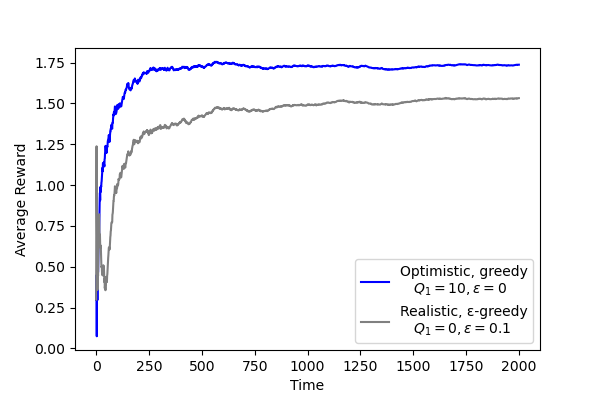
\includegraphics[width=0.75\linewidth]{images/optimistic.png}
    \caption{Comparison of Optimistic Initial Values}
    \label{fig:optimistic_greedy}
\end{figure}

\subsection{Upper-Confidence-Bound (UCB) Action Selection}

Exploration is needed because the agent is uncertain about the reward distributions of the bandits. The agent has to explore other bandits to learn their reward distributions and exploit the best-known bandit to maximize the total reward. The agent has to balance exploration and exploitation to maximize the total reward. The agent has to choose the perfect ratio of exploration and exploitation.

The Upper-Confidence-Bound (UCB) Action Selection Algorithm is one of the many solutions to the Exploration-Exploitation Dilemma. The agent selects the bandit with the highest upper confidence bound at each time step. The agent \textit{exploits} the best-known bandit by choosing the action with the highest upper confidence bound.

The action value of a bandit $a$ at time step $t$ is updated using the following formula:

\begin{equation}
    A_t \doteq \argmax_{a} \left[Q_t(a) + c\sqrt{\frac{\ln t}{N_t(a)}}\right]
\end{equation}

where $N_t(a)$ is the number of times the action $a$ has been selected prior to time $t$, and $c$ is a hyperparameter that controls the exploration and exploitation trade-off. A higher value of $c$ encourages more exploration, while a lower value of $c$ encourages more exploitation.
plt.savefig('report/images/ucb.png')

As can be seen in the Figure~\ref{fig:ucb}, the UCB Algorithm performs better than the Greedy Algorithm and the $\epsilon$-Greedy Algorithm. The agent explores other bandits to learn their reward distributions and exploits the best-known bandit to maximize the total reward.

\begin{figure}[h!]
    \centering
    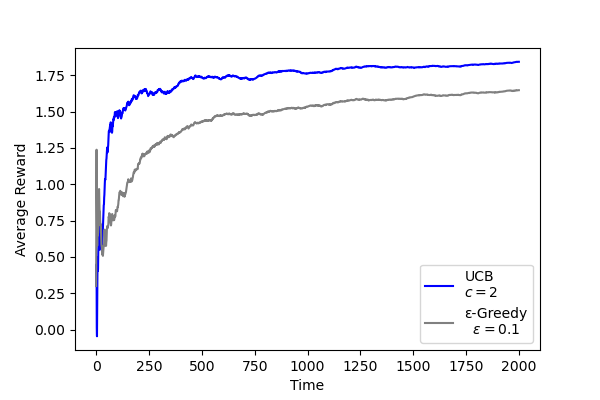
\includegraphics[width=0.75\linewidth]{images/ucb.png}
    \caption{The UCB Algorithm}
    \label{fig:ucb}
\end{figure}

% \subsection{Gradient Bandit Algorithm}

% \subsection{Associative Search (Contextual Bandits)}

% I skipped the above topics$\dots$ :P 

\section{Finite Markov Decision Processes}

This chapter introduces the concept of a Markov Decision Process (MDP) and its finite variant. We will define the MDP and its components, and discuss the optimal policy and value function. We will also introduce the Bellman equations and the value iteration algorithm, which are used to find the optimal policy and value function.

\subsection{The Agent-Environment Interface}

\subsection{Goals and Rewards}

\subsection{Returns and Episodes}

\subsection{Unified Notation for Episodic and Continuing Tasks}

\subsection{Optimality and Approximation}
\section{Dynamic Programming}

\subsection{Policy Evaluation (Prediction)}

\subsection{Policy Improvement}

\subsection{Policy Iteration}

\subsection{Value Iteration}

\subsection{Asynchronous Dynamic Programming}

\subsection{Generalized Policy Iteration}

\subsection{Efficiency of Dynamic Programming}
\section{Monte Carlo Methods}

Monte Carlo methods are a class of algorithms that rely on random sampling to estimate the value function. These methods assume that the sample is huge enough to provide a good estimate on the value of the state.

This method is better than the Dynamic Programming methods when the model of the environment is not known. And, the Monte Carlo techniques update the value function after the episode ends, unlike the Dynamic Programming methods which update the value function after each step.

\subsection{Monte Carlo Prediction}

The Monte Carlo Prediction is the process of estimating the value function of a policy by averaging the returns observed after visits to the stare. 

The Monte Carlo Predictions can be done in two ways:
\begin{itemize}
    \item \textbf{First-visit Monte Carlo}: The value of a state is the average of the returns following the first time the state is visited in an episode.
    \item \textbf{Every-visit Monte Carlo:} The value of a state is the average of the returns following every visit to the state in an episode.
\end{itemize}

The algorithm for First-visit Monte Carlo is as follows:

\begin{algorithm}
    \caption{First-visit Monte Carlo Prediction, for estimating V $\approx v_\pi$}
    \begin{algorithmic}
        \State Input: a policy $\pi$ to be evaluated
    \end{algorithmic}
    \begin{algorithmic}
        \State Initialize:
        \State $V(s) \in \mathbb{R}$, arbitrarily, for all $s\in\mathcal{S}$
        \State $Returns(s) \leftarrow$ an empty list, for all $s\in\mathcal{S}$
    \end{algorithmic}
    \begin{algorithmic}
        \While{True (for each episode)}
            \State Generate an episode following $\pi$: $S_0, A_0, R_1, S_1, A_1, R_2, \dots, S_{T-1}, A_{T-1}, R_T$
            \State $G \leftarrow 0$
            \State For each step of the episode $t=T-1, T-2, \dots, 0$:
            \State $G \leftarrow \gamma G + R_{t+1}$
            \If{$S_t$ not in $S_0, S_1, \dots, S_{t-1}$}
                \State Append $G$ to $Returns(S_t)$
                \State $V(S_t) \leftarrow \text{average}(Returns(S_t))$
            \EndIf
        \EndWhile
    \end{algorithmic}
\end{algorithm}

\newpage

\section{Plan of Action}

My plan of action for the remaining term is:

\begin{table}[h!]
\centering
    \begin{tabular}{ >{\centering\arraybackslash}m{3cm}>{\arraybackslash}m{12cm} }
        % \hline
        \rule{0pt}{2em}\textbf{Week} & \rule{0pt}{2em}\textbf{Plan} \\
        % \hline
        \rule{0pt}{2em}Week 6 & \rule{0pt}{2em}Monte Carlo methods \\
        % \hline
        \rule{0pt}{2em}Week 7 & \rule{0pt}{2em}Temporal-Difference \\
        % \hline
        \rule{0pt}{2em}Week 8 & \rule{0pt}{2em}Using RL techniques to make models that play games like Tic-Tac-Toe \\
        % \hline
        \rule{0pt}{2em}Week 9 & \rule{0pt}{2em}Using RL techniques to make models that play games like Tic-Tac-Toe \\
        % \hline
    \end{tabular}
\end{table}

% \begin{align*}
%     P(X_i|X_{\sim i}) &= \frac{P(X_i,X_{\sim i})}{P(X_{\sim i})} \\
%     &= \frac{\exp(-\sum_{c\in A_i}{V_c(x_c)}-\sum_{c \notin A_i}{V_c(x_c)})}{\int \exp(-\sum_{c\in A_i}{V_c(x_c)}-\sum_{c \notin A_i}{V_c(x_c)})dX_i} \\
%     &= \frac{\exp(-\sum_{c\in A_i}{V_c(x_c)\cdot\exp(-\sum_{c \notin A_i}{V_c(x_c)})})}{\exp(-\sum_{c\notin A_i}{V_c(x_c)})\cdot\int\exp(\sum_{c\in A_i}{V_c(x_c)})dX_i} \\
%     &= \frac{\exp(-\sum_{c\in A_i}{V_c(x_c)})}{\int\exp(\sum_{c\in A_i}{V_c(x_c)})dX_i} \\
%     &= P(X_i|X_{N_i})
% \end{align*}

\printbibliography

\printindex

\end{document}